\documentclass{article} %report?
%\usepackage{natbib} apa style etc.
\usepackage{amsmath}
\usepackage{verbatim}
\usepackage{subfigure}
\usepackage[pdftex]{graphicx}
\usepackage[english]{babel}
\usepackage[colorlinks=true, linkcolor=black, urlcolor=blue, pdfborder={0 0 0}]{hyperref}
%\usepackage{synttree}
%\usepackage[utf8x]{inputenc}

\title{Model Minimization in Qualitative Reasoning}
\author{Andreas van Cranenburgh \\ 0440949 \\ acranenb@science.uva.nl 
\and Hanne Nijhuis \\ 0364568 \\ hnijhuis@science.uva.nl}

\begin{document}
\maketitle

%perhaps picture here (something to do with minimization)

\vspace{15em}

\abstract{Qualitative Process theory provides a way of modeling causality in a
system on a qualitative level. Previous work has attempted to automatically
induce such qualitative models from behavior. We extend this work by turning
the resulting monolithic models into minimized, modular models, which makes
the induced models re-usable. The resulting minimization algorithm is general
enough to apply to user created models as well. We also sketch other possible
improvements for model induction, based on the exploitation of human
intuitions about systems rather than the current reliance on complete and
error-free data.}

\newpage

\tableofcontents

\newpage

\section{Introduction}

\section{Literature Review}

In this section we will review a few of the papers that have contributed
greatly to the definition of Qualitative Reasoning. We will give a short
summary of the papers and will conclude with an overview of the current field
of research and possible future work. 
%more text?

\subsection{Qualitative Reasoning}
Qualitative Reasoning is an approach from Artificial Intelligence that provides
means to express conceptual knowledge such as the physical structure,
causality, processes, etc.  This enables reasoning about phenomena for which
numerical information is sparse or missing, or when such information is too
complex to grasp.  The following papers describe the foundations of qualitative
reasoning.

\subsubsection{A qualitative Physics based on confluences (de Kleer \& Brown)}

De Kleer et al. \cite{kleer} present a framework for formalizing physics in a
manner that is {\em qualitative} rather than {\em quantitative}. Whereas
physicists describe the world in terms of continuous differential equations,
the rest of the world uses an implicit psychological model of naive physics.
The framework of \cite{kleer} falls between these two extremes of precision and
informality. They employ confluences, which are qualitative differential
equations.  Although their framework is completely qualitative, as opposed to
standard physics, on the other hand their framework is formal in the sense of
explicitly defining causal and structural relations, as opposed to the
psychological models of humans (presumably). Moreover, their approach is based
on deriving qualitative physics from first principles, like normal physics, as
opposed to the contextual and tacit knowledge of mere mortals.

This approach is presented as being useful for physics education, expert
systems and even physics, in that it explicitly deals with causality. The
latter is in contrast with standard physics, in which laws are merely
exceptionless correlations with predictive value. Although the mathematics
behind physics is relatively formal, doing physics depends on a pretheoretical
understanding of the world, of which there is no successful account to date
(neither in physics nor in psychology). Textbooks for physics and second
language learners clearly contain enough information for humans to grasp
such subjects (albeit only after intensive study), however, they are nowhere
formal (explicit) enough to be useful for the current computational paradigms;
they seem to rely on an extensive common ground.

Naive physics attempts the herculean\footnote{or foolish, depending on your
disposition} task of explicitly formalizing all the required knowledge to
derive fragments of modern physics in a qualitative manner. The fundamental
question at stake here is how deep the rabbit hole goes in terms of the
required background knowledge which is so much taken for granted by mortals.

A few assumptions of their approach characterize their methodology:

\begin{description}
	\item[No function in structure]
		The functioning of the whole should not be encoded in its
		parts. For example, a light switch should not state that it
		directly determines whether there will be light, because other
		things such as the state of the light bulb and the payment of
		bills also influence such matters, let alone the need for a
		closed circuit.

	\item[Class-wide assumptions]
		Modeling always happens at a certain resolution yielding a
		level of description. Brownian motion, quantum entanglement
		and other quaint microcosmic phenomena can be safely ignored
		not just for certain models, but for any model which aims for
		the same predictive power as human folk physics. The modeling
		granularity also includes time and spatial resolution; for
		example oscillation phenomena is ignored as long as the system
		needs only a certain negligible amount of time to settle.
	
	\item[Locality]
		This principle states that the behavior of parts cannot
		influence other parts, except when they are structurally
		connected. This is strongly related to the focus on causality,
		and implies that without a locus of causality there can be no
		model (eg., an emergent phenomenon like a tornado could not be
		modelled).

	\item[The importance of principles]
		Violating the first principle has no result on the success
		of accurately modeling certain behavior, but it does result in
		ad-hoc models with little value for understanding actual
		physics. This is comparable to the situation of observing a
		mere correlation without positing a plausible causal mechanism;
		this provides no information whatsoever about possible
		causality and does not further understanding -- it is a
		pointless exercise in data collection.

		This fine point is easily glossed over when the goal of
		deriving first principles fades out of sight; without
		principles hacking together models is pointless, because one
		will simply continue until the desired output is there, but if
		the desired output was clear to begin with, it is impossible
		for a model to add any value.
\end{description}

Advantages of this approach are that it works from first principles, so it is
grounded in science. Other advantages are that the models can be induced from
data, even when it contains noise. Disadvantages are that these constraint
models are less explanatory than process models (\cite{forbus}, p. 110), 
which we will review promptly.

\subsubsection{Qualitative Process Theory (Forbus)}

Around the same time as de Kleer \& Brown, another approach was introduced by
Forbus \cite{forbus}. The important points that set his work appart were,
among others, the \emph{quantity-spaces} and the \emph{sole mechanism
assumption}.

The principle of quantity spaces represents values by a set of ordinal
relationships. This enables the system to easily compare the different
quantities in terms of smaller, equal or larger. If such comparisons would
only occur between two values, then sign values would suffice (-,0,+), but for
many cases, the ordinal representation is more natural.

\vspace{0.8em}

Physical processes are viewed as the mechanisms through which change occurs.
To this end Forbus introduced the \emph{sole mechanism assumption} which
states that any behavior must be explainable by the direct or indirect effects
of some collection of physical processes.

\vspace{0.8em}

Forbus has reviewed his own work and the impact of his work in
\cite{forbus12}.
%more text

\subsubsection{Mediating conceptual knowledge using qualitative reasoning}

Capturing conceptual models can show the consequences of what we believe to be
true, analogous to formal logic. Using computer simulations large models can
be evaluated, showing the interactions of fragments of knowledge. The rest
of the text deals with Garp which is discussed in the next section.

In the introduction it is claimed that:

	``Qualitative models excel when theoretical background on the target
	system is weak, when the problems are ill-defined, and when data are
	incomplete.''

This statement is unfortunately not backed up by {\em any} supporting evidence.
Phrased like this it would seem that qualitative models provide us with a brave
new kind of science, which is in fact false, unless one trivializes the claim
to ``scientists implicitly use qualitative models to do science.'' What in fact
would seem to be the case is that qualitative models provide a formalization
of knowledge, and as such, require that this knowledge is perfect: complete,
consistent and enumerable; otherwise formalization will grind to a halt
immediately, because resolving inconsistency already presupposes a proper
understanding. The way humans deal with inconsistency is an interesting topic
in itself, but suffice to say that the quoted passage is most likely very far
from the truth.

\subsubsection{Garp3 - Workbench for Qualitative Modeling and Simulation
(Bredeweg et al.)}

Garp3 is an implementation of Qualitative Process Theory with a focus on
educational uses.

Tools are being build to take a graphical approach to building qualitative 
models. With the introduction of Garp3, Bredeweg et al. want to preserve the
full expressiveness of the QR formalism and to address domain experts and
support them in articulating and capturing their conceptual knowledge. The
software uses a diagrammatic approach for representing model content.

In Qualitative Reasoning, quantities that describe the dynamic features of a 
system typically hold qualitative information concerning the current magnitude 
and direction of change, using an interval scale, consisting of an ordered set 
of labels, e.g. {zero, low, medium, high}. such a set of labels
is called a quantity space. Landmarks are specific labels within this set
(acutally points) that refer to situations in which the behaviour of the system
changes significantly. For instance, a susbstance reaching its boiling
tempurature will stop getting hotter and start boiling. In qualitative
simulations, the behavior of the system is represented as a graph of states
that reflect qualitatively distinct system behavior. There is a set of
dependencies that capture cause-effect relationships between quantities,
defined in such a way that they are both closely resembeling the conceptual
notions of human reasoning, as well as allowing automated computation because
they are grounded in mathematical formalisms. Two typical dependencies are
direct influences and proportionalities.

A QR engine has inference mechanisms to assemble the appropriate set of
dependencies that describes a system in a certain state of behaviour. Two
aspects are important for this approach: behaviour can be inferred from the
physical structure of the system, and knowledge about system behaviour is
stored in small fragments with conditional information detailing when such a
fragment is applicable.

\vspace{0.8em}

Simulation is done by the Garp3 reasoning engine, using a state-by-state
strategy. The \emph{find-states} algorithm constructs initial nodes in the 
state-graph based on the scenario and model fragments. Then the 
\emph{find-transitions} algorithm determines all possible changes which form 
transition scenarios. These are inputted into the find-states procedure again.  

The reasoning process relies heavily on inequality reasoning.
The mathematical engine inequality relations typically change during the 
simulation, thereby representing the dynamic aspects of the modelled system. 
Points in a quantity 
space are called landmarks and the intervals between are defined by these
landmarks. The core inequality reasoning only considers these landmarks and not
the intervals. Inequalities can specify the relation between several types of
model ingredients. The following five types of inequality relations are used in
Garp3: \emph{Quantity} $\leftrightarrow$ \emph{Quantity}, \emph{Quantity} 
$\leftrightarrow$ \emph{Landmark}, \emph{Landmark} $\leftrightarrow$ 
\emph{Landmark}, \emph{Derivative} $\leftrightarrow$ \emph{Derivative}, 
\emph{Derivative} $\leftrightarrow$ \emph{Zero}.  

At the user-level representation, quantity values, landmarks and derivatives are
used, while at mathematical level, only landmarks exist and are used to
describe the others (for both magnitudes and derivative quantity spaces).

All the relations in the internal mathematical model of Garp3 have the
following form: $Sum_1$ $rel$ $Sum_2$ with $rel \rightarrow \{>,\ge,=\}$. The following
three basic principles are used to make inferences in the Garp3 inequality
reasoning engine:

\begin{itemize}
\item Bais algembraic simplification
\item Anti-symmetry
\item Transitivity
\end{itemize}
For example:
\begin{itemize}
\item $A>B$, $B>C$ (given)
\item $(A>B)\&(B>C) \rightarrow A+B>B+C$ (transitivity)
\item $A+B>B+C \rightarrow A>C$ (simplification)
\end{itemize}

Garp3 does not discriminate explicitly between inequality statements that
should be treated as always true (e.g. \emph{inflow} - \emph{outflow} = 
\emph{net-flow}), and those that may change during simulation 
(eg. $T_x < T_xboil \rightarrow T_x = T_xboil$).

\vspace{0.8em}

2nd order derivatives are important for sound simulations, but complete
validity cannot be guaranteed. This issue is in principle unsolvable, but does
not form a problem for the level of detail of models built in Garp3.  

Future work will focus mainly on improving usability of the software in terms
of GUI and debugging options.

Bredeweg et al. conclude that the Garp3 workbench offers easy access to 
sophisticated qualitative simulation software, providing users the 
possibility to use QR technology withou having to understand low-level 
implementation details of such automated reasoners. An increasing number of 
domain experts are using the workbench to capture qualitative knowledge of 
system dynamics.  

\subsubsection{Algal bloom in the Danube Delta (Cioca et al.)}

A Garp model of a system in the ecological domain, demonstrating its
applicability to the formalization of real-world problems.

%more to come

\subsubsection{Discussion}

The idea that Qualitative Reasoning can formalize actual common sense knowledge
and human understanding of physics is by now outdated. It is an instance of the
``Good Old Fashioned Artificial Intelligence'' (GOFAI) approach,
\cite{haugeland} and in line with the Symbol System hypothesis of Newell and
Simon \cite{newell}\footnote{``A physical symbol system has the necessary and
sufficient means of general intelligent action.''}.  Both of these have either
failed spectucularly or faded silently, often having been replaced by
stochastic and data-driven approaches \cite{russellnorvig}.  Claiming that
Qualitative Reasoning can provide a way to model actual common sense knowledge
or mental models is ostensively wrong -- the list of mismatches with human
intuitions is unmanageble, and among these mismatches are the parts where Folk
% cite examples from class/literature?
Physics is ostensively {\em wrong}. Specifically philosophers contend that
common sense is holistic at its core \cite{smith}, whereas explicit,
knowledge-based approaches are reductionistic in nature, because their aim is
to isolate context-free fragments. 

Therefore we submit that it is no longer useful to present it as a part of
Artificial Intelligence or having anything to do with common sense; while QR
models are certainly artificial, they are not in the least intelligent, nor are
they common or do they make sense to non-experts.  They are simply an explicit
formalization of a certain set of behaviors of interest. This does not mean
that Qualitative Reasoning is itself a fruitless enterprise -- it can be used
as an educational tool, where there is no need for bold philosophical claims.

With this educational focus in mind it makes sense to try to facilitate the
modeling process for non-experts for which QR is useful. To this end we turn
to the topic of model induction.

\subsection{Automated Modeling} %Automated or automatic?

To introduce the recent developments in the field of automated modeling we
will now review a few papers on this topic.

\subsubsection{Automated modeling in process-based qualitative reasoning
(Buisman)}

The concept of automated modeling for qualitative process theory was
introduced by Buisman \cite{buisman} in 2007. He motivates the research with
the goal to relieve the strain placed on experts and beginners, and to speed
up the modeling process. The approach he took however, does not attain these
goals yet, but is more of an exploration of the possibilities of using
Artificial Intelligence to induce models based on behavior graphs. We will
give a short overview of the algorithm he developed.

The input for the algorithm consists of:

\begin{itemize}

\item Behavior graph (states and state transitions) of a full envisionment

\item Scenario (partial information about structural relations between entities and their quantities)

\item ISA-hierarchy (full description of entity type hierarchy and quantities)

\end{itemize}

With this input, the algorithm produces models which are ready for simulation.
For each scenario they should give the same output as the original model.

There are certain constraints on the input. The \emph{full envisionment}
requirement means that the behavior is known for all possible initial values
for all quantities in the system. Also, the derivatives and amounts have to be
defined for every state. Finally, the input data cannot contain any noise,
ie., it should be perfect.

The algorithm starts with searching for so called \emph{naive dependencies},
which are dependencies that are consistent with the entire state-graph. They
are found by applying consistency rules on all pairs of quantities. These
consistency rules consider the amount and derivative values of the quantities
for all states, so as to induce possible dependencies. For example, a positive
influence between $Q_1$ and $Q_2$ could exist if for every state $A_s(Q_1) =
D_s(Q_2)$.  There will be redundancy in the set of naive dependencies which
has to be pruned by filtering out substitutionary groups, which are defined as
mutually exclusive possible disambiguations. 

%HAVE TO REWRITE THIS!!
%testing.. 

\subsubsection{Jochem}

Actuators

%more text

%less brute force, instead attempt to find the conceptually correct model
%immediately; added a knowledge base of actuators: common patters etc.

\subsubsection{Carsten}

%more text

Causal groups % feedback loops, interacting processes

\subsection{Overview}

%overview of what?


\newpage
%\chapter{Project} needs report document class

\section{Theory}

In the field of QR, models %( / scenario's / systems ?) 
consist of several smaller fragments which can be roughly divided in three
categories: static, process and agent. This categorization is not strict, but
gives a certain view on how things work. Static fragments are used to describe
the structure of a model, as well as proportionalities between quantities. A
static fragment cannot have any agents or influences in it. A \emph{process}
fragment should have at least one direct influence and is not restricted in
terms of dependencies. %(relations?)
Finally, \emph{agent} fragments should be used to describe any influences on a
system that are external, hence not part of the system itself.

Fragments can be useful to make the complete system more comprehensible --
ie., they are a form of chunking.  Also, while building these complex models,
fragments allow the user to focus on what happens in a small part of the
model, without having to worry about the other 'components'. For example in a
model describing a population, seperate fragments could describe processes
like birth, death, emigration, etc.
%maybe reference to paper BredewegEtAl, they say fragments are important in QR

Recent work on automated modeling \cite{buisman, liem, vanweelden} has focused
on generating a correct model based on a full-envisionment behavior graph. The
current algorithms always produce a single model fragment which describes the
complete system. The implicit compositionality of a system is not revealed and
comprehending the output could become quite difficult with large models. We
therefore introduce a way of splitting and minimizing such monolithic models
into smaller fragments while preserving the exact same behavior.

See figure \ref{pipeline} for an overview. %more text.

\begin{figure}[ht]
\centering
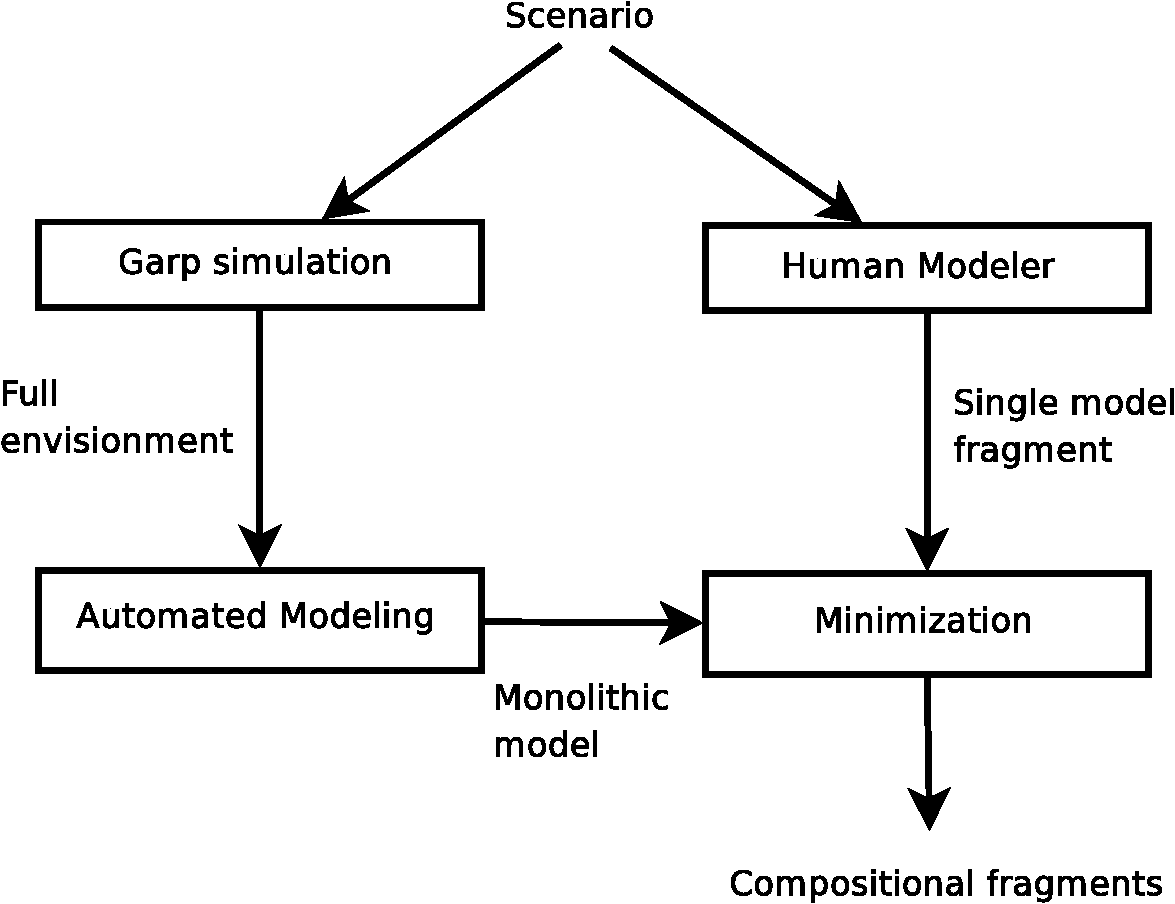
\includegraphics[scale=0.5]{pipeline-crop.pdf}
\caption{The pipeline of operations and relation to previous work.}
\label{pipeline}
\end{figure}

\subsection{Interdisciplinary parallels}

%\item Parsimony, Occam's razor (philosophy of science)
%wrong, parsimony refers to most simple explanation, not representation

\subsubsection{Finite-State automaton miniminization, compression}

	In automata theory there are well-known results regarding the
	minimization of grammars. For example there exists an algorithm to
	obtain a minimized version of a Finite-State automaton (FSA) which
	generates the exact same language with a minimum amount of states
	\cite{hopcroft}.

	Naturally this problem gets more difficult (no general purpose
	algorithms exist) higher up in the Chomsky hierarchy, so it would be
	an important result if it turned out that (a subset of) qualitative
	model simulation can be encoded as a Finite-State automaton that
	generates a regular language containing state-strings corresponding to
	behavior paths.

	A related but less hopeful result is that of Kolmogorov complexity,
	which states that given an arbitrary string, it is undecidable to
	verify whether a given program generating that string is the shortest
	one to do so (ie., highest compression), let alone to produce such a
	program given data.

	Determining the exact status of qualitative reasoning with respect to
	established results in automata theory or formal logic would shed light
	on the precise complexity and feasibility of model induction.
	%This is analogous to our goals.

\subsubsection{Minimum Description Length principle}

	In Machine Learning there is the Minimum Description Length (MDL;
	\cite{mitchell}, p. 171, section 6.6)
	principle, which provides an inductive bias to choose among possible
	hypotheses for data, given a certain representation (the latter is
	crucial to success).  This provides a powerful heuristic because
	whenever a hypothesis is found that fits the data, all larger
	hypotheses can be discarded.
	
	If we apply this principle to qualitative model induction, then
	minimizing a model that fits the data will yield a better hypothesis
	according to the MDL principle.
  
\subsubsection{Economy of Representation (Generative Linguistics)}

	This principle states that representations are non-redundant. The
	abstract representation of a surface form like ``the boys walk'' will
	only contain the feature \textsc{plural} once, because agreement in
	number between the subject and verb is mandatory, and hence there is
	no point in storing the feature twice. 

	Similarly when a scenario in a qualitative model contains two trees,
	both should rely on one and the same dependency stating the relation
	between size and shade, not on two dependencies specific to their
	instances. 

\section{Approach}

In this section we describe our approach on minimizing, generalizing and
splitting single model fragments into modular and compositional fragments.
First the problem will be stated, then an algorithm, and finally some promising
results.
%more text

\subsection{Problem statement}

We take a monolithic model and divide it into several smaller fragments. To do
so, we need to comply to the following ranked list of
constraints:\footnote{Note that the terminology in this section of ranked
constraints, candidates and optimality is of course a nod to Optimality
Theory \cite{princesmolensky}}

\begin{enumerate}
\item The model should be equivalent, that is, the resulting behavior should
	be exactly the same as the original given the same input (a scenario).

\item The output should be as parsimonious as possible, that is, fragments
	should be minimal.

\item General fragments are preferred over specific fragments; this entails a
	bias for smaller fragments and modularity.

\end{enumerate}

We make no claim as to the didactic and cognitive suitability of these
constraints, but it is not hard to imagine that these constraints will provide
an improvement when applied to any model lacking in modularity. It is well
known that modularity is a sound engineering approach, and there is no reason
to assume Qualitative Reasoning to be an exception. However, there are subtle
choices to be made as to the exact granularity of fragments, because these
constraints underdetermine the space of candidates, and because cognitive
optimality would demand empirical studies about chunking and comprehension
etc. We will gloss over these issues and apply the aforementioned constraints
without further claims of optimality.

\subsection{Algorithm}

Overview:

\begin{itemize}

\item Find a list of pivots, conditions on which the model fragments are
	based. Currently these are single structural relations.

\item For each pivot, find a set of dependencies which apply whenever the
	pivot is present, without exception

\item Generalize these dependencies into a single model fragment, several
	dependencies among instances may be collapsed into one

\end{itemize}

% fragments that can be generalized (ie., relations between quantity classes)
% collapes M into a set of sets containing generalized dependencies.
%
% incorrect definition (todo): fragments = smallest union of all possible sets
% { d | dependency(d) & d = generalized(di) & di in M } such that there is
% exactly one structural relation shared by them.
%
% where dependency is true for dependency triples, and generalized is a
% function that takes a dependency between instances of quantities and returns
% a dependency between the classes of those entities.

Sketch of the algorithm:

\begin{enumerate}

\item Input: take the set of dependencies, $M$, (as generated by eg. model
	induction or from a monolithic model fragment created by a user).  

\item Partition this set into equivalence classes according to the
	equivalence relation of the conditions under which each dependency
	holds.

\item Minimize each equivalence class by substituting 
	$Q_1 \overset{I+}{\rightarrow} Q_2 $ for a set such as 
	$ \{ Q_1^a \overset{I+}{\rightarrow} Q_2^b, Q_1^c \overset{I+}{\rightarrow} Q_2^d,  . . . \} $, 
	yielding elements of the set $MFs$

\item Dump the remaining dependencies in a single fragment, $UF$. 
	This set should be empty if the model is properly designed, ie., the
	model should not contain dependencies that apply to some instances but
	not to others.

\item Output: minimized model $ = MFs \cup \{ UF \} $

\end{enumerate}

This sketch can be formalized and instantiated into a definition with set
builder notation.\footnote{Note that the following definitions closely follow
our Prolog implementation, as such they include certain choices and
simplifications limiting the generality of the approach as previously
sketched.}  First two helper definitions. The first definition defines a
predicate for instances of structural relations and related quantities:

\begin{align*}
instance(R, E_1, E_2) :=
	\exists e_1, e_2 \; [ &struct\_rel(R, e_1, e_2) & \\
	\land \; &isa(e_1, E_1) \land isa(e_2, E_2) ]
\end{align*}
	
\begin{align*}
qinstance(R, Q_1, Q_2, q_1, q_2) :=
	\exists e_1, e_2 \; [ &struct\_rel(R, e_1, e_2) & \\
	\land \; &has(e_1, q_1) \land has(e_2, q_2)  \\
	\land \; &isa(q_1, Q_1) \land isa(q_2, Q_2) ]
\end{align*}

In this definition $q_n$ refers to an instance of a quantity $Q_n$, similarly
$e_n$ refers to an instance of an entity $E_n$; such pairs are related by the
$isa(a, b)$ predicate denoting that $a$ is an instance of $b$. Quantities and
entities are related by $has(e_n, q_m)$ denoting that $e_n$ has the quantity
$q_m$. Finally $struct\_rel(R, e_n, e_m)$ denotes the configuration that $e_n$
is structurally related to $e_m$ with relation $R$; for practical purposes
we assume that each entity has a reflexive relation called ``self,'' which
allows the isolation of dependencies between the quantities of a single
entity.\footnote{see the communicating vessels for an example with amount,
height and pressure of a container} %idea, besides implicit self relation,
%perhaps add unconditional relation holding between any two entities so that
%com.ves. can be splitted without an unfragment. but: relation is not unconditional, but a combination of two relations: vessel 1 and 2 are both connected to the same pipe, with from and to respectively.

The next definition defines an equivalence relation on these instances,
stating that their dependencies hold universally given their condition (which
is here restricted to a single structural relation):

\begin{align*}
samedeps(R, E_1, E_2, M) := \\
	\; \forall d, q_1, q_2 \; [ \; 
	(&dependency(d, q_1, q_2) \in M \\
	\land \; &qinstance(R, E_1, E_2, q_1, q_2, Q_1, Q_2)) \\
	%\land \; &isa(q_1, Q_2) \land isa(q_2, Q_2) \\ 
	%\land \; &has(q_1, e_1) \land has(q_2, e_2) \\
	%\land \; &isa(e_1, E_1) \land isa(e_2, E_2) ) \\
	& 	\rightarrow \forall e^\prime_1, e^\prime_2 \; [ \;
	 qinstance(R, E_1, E_2, q^\prime_1, q^\prime_2, Q_1, Q_2) \\
	%( isa(e^\prime_1, E_1) \land isa(e^\prime_2, E_2)  \\
	%&	\quad 	\land struct\_rel(r, e^\prime_1, e^\prime_2)  \\
	%&	\quad 	\land has(e^\prime_1, q^\prime_1) \land has(e^\prime_2, q^\prime_2) ) \\
	& \qquad \rightarrow dependency(d, q^\prime_1, q^\prime_2) \in M \; ] \; ]
\end{align*}

Here $dependency(d, a, b)$ denotes a directed relation $d$ between $a$
and $b$ (undirected relations can be expressed using two directed relations).
Possible values for $d$ correspond to influences, proportionalities,
correspondences and equalities. While $a$ and $b$ usually denote quantities,
note that they can also refer to an arithmetic operation between two
quantities, eg. $min(q_n, q_m)$.

These two predicates combined give us the set of pivots for a given
monolithic model:

\begin{align*}
qpivots := \{ \; \langle R, Q_1, Q_2 \rangle \; | \\
	\; &qinstance(R, Q_1, Q_2, q_1, q_2) \\
	\land \; &isa(q_1, Q_1) \land isa(q_2, Q_2) \\
	\land \; &has(E_1, Q_1) \land has(E_2, Q_2) \\
	\land \; &samedeps(R, E_1, E_2, M) \} 
\end{align*}

Instead of defining pivots on pairs of quantities, we can also use pairs
of entities:

\begin{align*}
epivots := \{ \; \langle R, E_1, E_2 \rangle \; | 
	\; instance(R, E_1, E_2) 
	\land samedeps(R, E_1, E_2, M) \} 
\end{align*}

After defining the pivots we simply map them to their dependencies to obtain
minimized, modular fragments:

\begin{align*}
qfragments := \{ \; \{ \; dependency&(d, Q_1, Q_2) \; | \; \\
		& dependency(d, q_1, q_2)  \in M \\
		& isa(q_1, Q_1) \land isa(q_2, Q_2) \} \\
	\; | \; \langle R, Q_1, Q_2 \rangle &\in qpivots \lor 
	\langle R, Q_2, Q_1 \rangle \in qpivots \; \}
\end{align*}

Similarly for pivots of pairs of entities:

\begin{align*}
efragments := \{ \; \{ \; dependency&(d, Q_1, Q_2) \; | \; \\
		& qinstance(R, E_1, E_2, q_1, q_2, Q_1, Q_2) \\
		\land \; & dependency(d, q_1, q_2)  \in M \} \\
	\; | \; \langle R, E_1, E_2 \rangle &\in epivots \lor 
	\langle R, E_2, E_1 \rangle \in epivots \; \}
\end{align*}

Note that while in this definiton pivots are restricted to single triples of a
relation and two quantities, the definition should be generalized so that
pivots can be merged into multiple triples when they are applicable under the
same conditions. This is in fact what we have done in our implementation,
where we derive pivots in a bottom-up fashion for the dependencies that remain
after the first pass of finding single condition pivots.

The communicating vessels model provides an example (see figure \ref{cv_mono}),
here there is a dependency between two containers, even though they are not
directly connected by a single structural relationship, but instead through
a mutual connection to the same pipe. Our algorithm tries to find a path of
structural relations between the two entities connected by the dependency in
question. This is not as simple as allowing for transitive connectivity,
because direction plays no role, and because cycles should be detected. The
shortest path is always used as the pivot.

\section{Results}

The evaluation is based on a few well known example Garp models. Initially
we wanted to use the output of the AM algorithm directly, but we experienced
some problems with the implementations of the AM algorithm.  The output of the
automatic modeling implementations of \cite{buisman} and
\cite{vanweelden} is not easily accessible in a simple prolog list. The output
of \cite{buisman} is sent directly to a new Garp model, which makes testing
easy, but the latest implementation \cite{vanweelden} which supports
interacting processes does not return equalities and arithmetic relations among
its output. The scenario and entity hierarchy is accessible through the Garp
API.
%FIXME remove this whining and hack a garp interface together.

To avoid having to deal with these implementation matters we have based our
current proof of concept implementation on our own Prolog representation. Our
implementation expects as its input a flat list of dependencies, and as
background knowledge the scenario and entity hierarchy. Because of this the
evaluation had to be done manually. We induced the models using the
implementation of \cite{buisman} so as to obtain monolothic models. An
advantage to this is that we could choose the conceptually correct direction of
proportionalities, which cannot be determined from the data using induction, as
noted by \cite{vanweelden}.

%\subsection{Evaluated Models}

\subsection{Tree and shade growth} 
% maybe show scenario with three trees, number of model fragments should stay the same! proof of concept.

When the tree \& shade model is splitted, the output remains a single model
fragment, because there is only one entity. If however one splits on the basis
of pairs of related quantities instead of on pairs of related entities, one
obtains the fragments as in figure \ref{ts_frags}, given the input as in figure
\ref{ts_mono}.

When a model of the full envisionment of a scenario with $n$ trees is induced,
the minimization algorithm will generalize this to the exact same fragment as
for a single tree.

%Input in figure \ref{ts_mono} and output in figure \ref{ts_frags}.
%more text

\begin{figure}[ht]
\centering
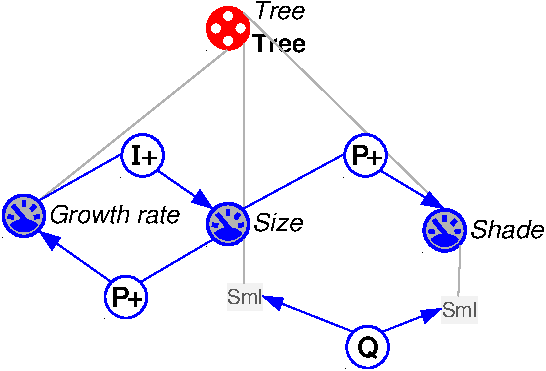
\includegraphics[scale=0.5]{ts_mono-crop.pdf}
\caption{Monolithic model as input}
\label{ts_mono}
\end{figure}

\begin{comment}
\begin{verbatim}
Input: 
[dependency(inf_pos, growth_rate1, size1), 
dependency(prop_pos, size1,growth_rate1), 
dependency(prop_pos, size1, shade1),
dependency(q_correspondence, size1, shade1), 
dependency(q_correspondence, shade1, size1)]

Set of struct rels: 
[ (self, size, size), (self, shade, size), (self, shade, shade), 
(self, growth_rate, size), (self, growth_rate, shade), 
(self, growth_rate, growth_rate)]
\end{verbatim}
\end{comment}

\begin{figure}[ht]
\centering
\subfigure{
    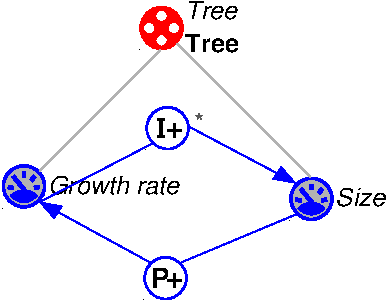
\includegraphics[scale=0.5]{ts_growth-crop.pdf}
}
\subfigure{
    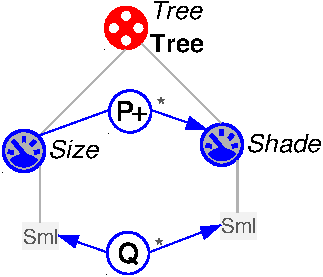
\includegraphics[scale=0.5]{ts_sizeshade-crop.pdf}
}
\caption{After minimization: two model fragments for growth and size of shade}
\label{ts_frags}
\end{figure}

\begin{comment}
\begin{verbatim}
Fragments (2): 
[ (self, shade, size), 
	dependency(prop_pos, size, shade),
	dependency(q_correspondence, size, shade), 
	dependency(q_correspondence, shade, size)] 
[ (self, growth_rate, size),
	dependency(inf_pos, growth_rate, size),
	dependency(prop_pos, size, growth_rate)]

Unfragment: []
\end{verbatim}
\end{comment}

\subsection{Stacked bath tubs}

For the stacked bath tub model we changed the quantity space of flow to ZPM
(instead of ZP) because this makes it possible to replace the
value-correspondences by a single Q-correspondence. Value correspondences are
not yet supported by the AM algorithm \cite{vanweelden}.  

The algorithm correctly splits the model into two fragments, equivalent to the
original model. For the input, see figure \ref{sb_mono}; for the output, see
figure \ref{sb_frags}.
%more text


\begin{comment}
\begin{verbatim}
Input: 
[dependency(inf_pos, flow12, level12), 
dependency(inf_pos, flow11, level11), 
dependency(inf_neg, flow12, level11), 
dependency(prop_pos, level11, flow12), 
dependency(q_correspondence, level11, flow12)]

Set of struct rels: 
[ (self, flow, flow), (self, level, level), (in, flow, level), 
(out, flow, level)]

Fragments (2): 
[ (in, flow, level), dependency(inf_pos, flow, level)]
[ (out, flow, level), 
	dependency(inf_neg, flow, level), 
	dependency(prop_pos, level, flow), 
	dependency(q_correspondence, level, flow)]

Unfragment: []
\end{verbatim}
\end{comment}

\begin{figure}[ht]
\centering
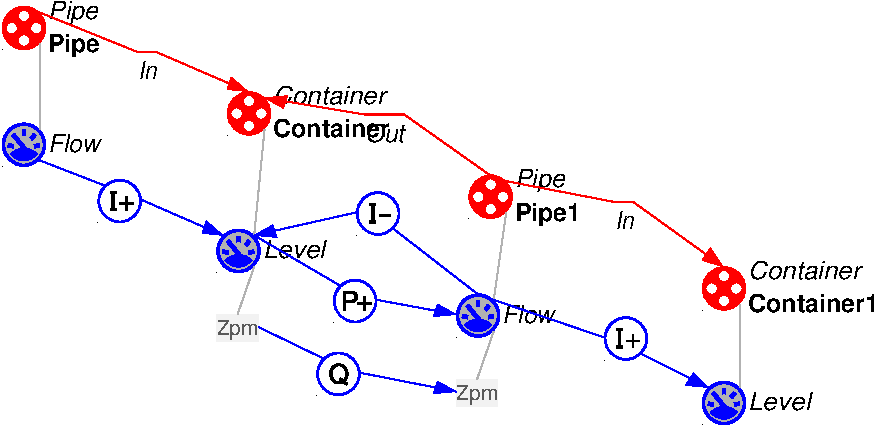
\includegraphics[scale=0.5]{sb_mono-crop.pdf}
\caption{Monolithic bath tub model as input}
\label{sb_mono}
\end{figure}

% -----


\begin{figure}[ht]
\centering
\subfigure{
    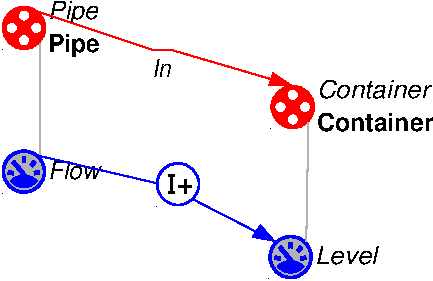
\includegraphics[scale=0.5]{sb_in-crop.pdf}
}
\subfigure{
    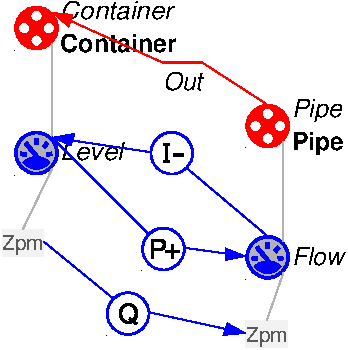
\includegraphics[scale=0.5]{sb_out-crop.pdf}
}
\caption{After minimization: two model fragments for flows going in and out respectively.}
\label{sb_frags}
\end{figure}

\subsection{Communicating vessels} 

The most complicated model we have tested is the fully compositional
communicating vessels model. Inducing the communicating vessels model almost
works, but for some reason one equality (between height and pressure) is not
found by the AM algorithm, so it has been added manually.  The algorithm
correctly minimizes the model into four fragments, no matter how many vessels
are in the scenario. This implies that the output is truly compositional.

For the input, see figure \ref{cv_mono}; for the output minimized using
quantities, see figure \ref{cv_frags}, figure \ref{cv_frags2} shows the output
minimized using entities.

%FIXME: is this really true? or is it only because Carsten's equalities are
%asserted god knows where?
%more text


\begin{figure}[ht]
\centering
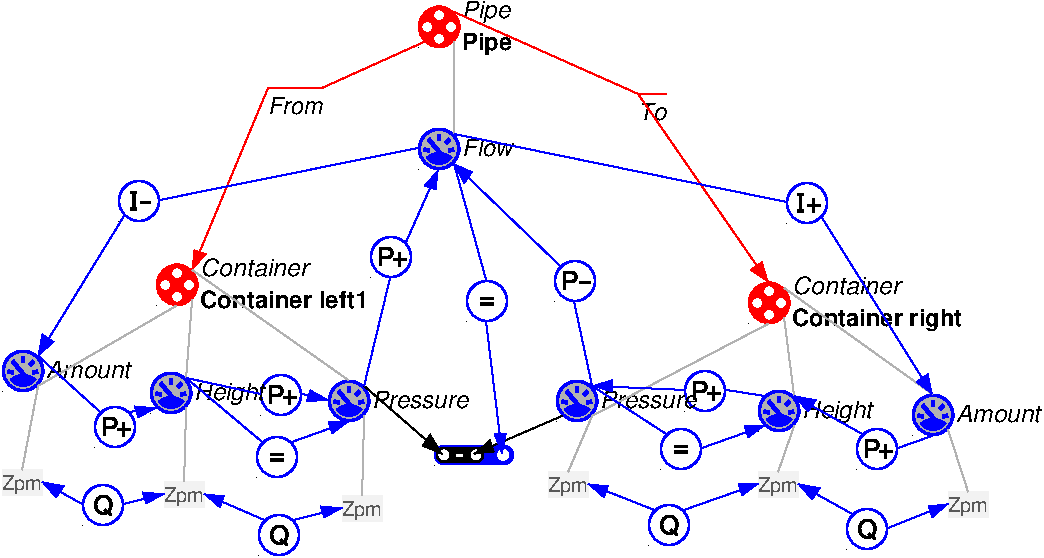
\includegraphics[scale=0.5]{cv2_mono-crop.pdf}
\caption{Monolithic model for two communicating vessels as input}
\label{cv_mono}
\end{figure}


\begin{figure}[ht]
\centering
\subfigure{
    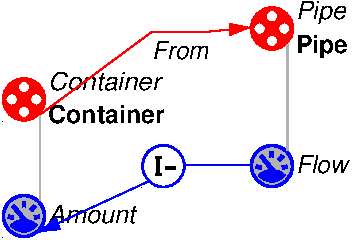
\includegraphics[scale=0.5]{cv_amountflow-crop.pdf}
}
\subfigure{
    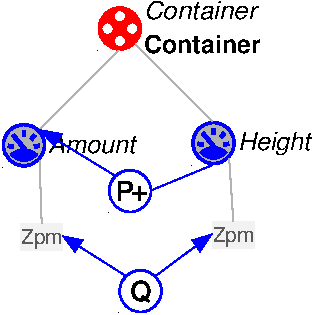
\includegraphics[scale=0.5]{cv_amountheight-crop.pdf}
}
\subfigure{
    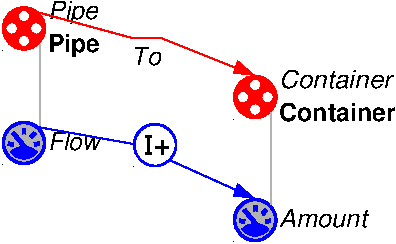
\includegraphics[scale=0.5]{cv_flowamount-crop.pdf}
}
\subfigure{
    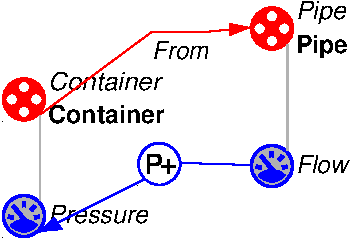
\includegraphics[scale=0.5]{cv_pressureflow-crop.pdf}
}
\subfigure{
    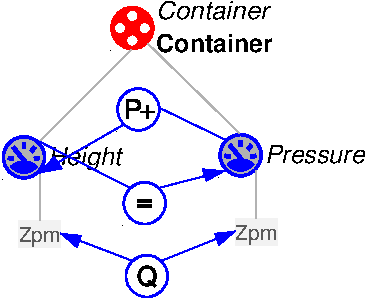
\includegraphics[scale=0.5]{cv_heightpressure-crop.pdf}
}
\subfigure{
    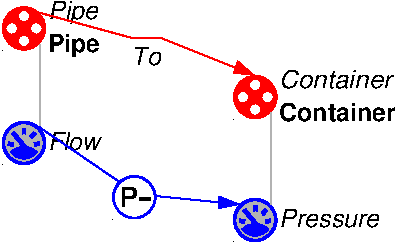
\includegraphics[scale=0.5]{cv_flowpressure-crop.pdf}
}
\subfigure{
    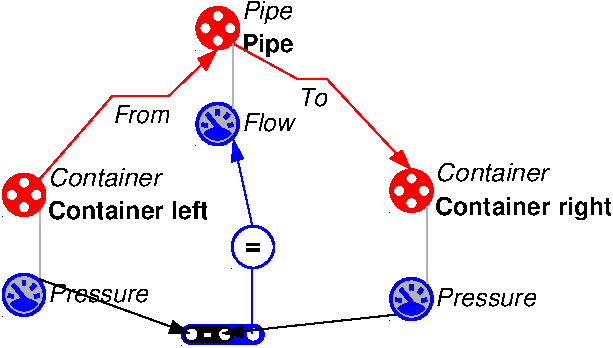
\includegraphics[scale=0.5]{cv_unfragment-crop.pdf}
}

\caption{After minimization on quantities: seven model fragments for two communicating vessels.}
\label{cv_frags}
\end{figure}

\begin{comment}
Two communicating vessels:

\begin{verbatim}
Input: 
[dependency(inf_pos, flow3, amount5), 
dependency(inf_neg, flow3, amount4), 
dependency(prop_neg, flow3, pressure5), 
dependency(prop_pos, flow3, pressure4), 
dependency(prop_pos, height4, amount4), 
dependency(prop_pos, height5, amount5), 
dependency(prop_pos, pressure5, height5), 
dependency(prop_pos, pressure4, height4), 
dependency(q_correspondence, height5, amount5), 
dependency(q_correspondence, pressure4, height4), 
dependency(q_correspondence, pressure5, height5), 
dependency(q_correspondence, height4, amount4), 
dependency(equals, flow3, min(pressure4, pressure5)), 
dependency(equals, height4, pressure4), 
dependency(equals, height5, pressure5)]

Set of struct rels: 
[ (self, flow, flow), (self, amount, amount), (self, amount, height), 
(self, amount, pressure), (self, height, height), (self, height, pressure),
(self, pressure, pressure), (from, amount, flow), (from, height, flow), 
(from, pressure, flow), (to, flow, amount), (to, flow, height), 
(to, flow, pressure)]

Fragments (6):
[ (self, amount, height), 
	dependency(prop_pos, height, amount), 
	dependency(q_correspondence, height, amount)]
[ (self, height, pressure), 
	dependency(prop_pos, pressure, height), 
	dependency(q_correspondence, pressure, height), 
	dependency(equals, height, pressure)]
[ (from, amount, flow), dependency(inf_neg, flow, amount)]
[ (from, pressure, flow), dependency(prop_pos, flow, pressure)]
[ (to, flow, amount), dependency(inf_pos, flow, amount)]
[ (to, flow, pressure), dependency(prop_neg, flow, pressure)]

Unfragment: [dependency(equals, flow3, min(pressure4, pressure5))]
\end{verbatim}
\end{comment}

\begin{figure}[ht]
\centering
\subfigure{
    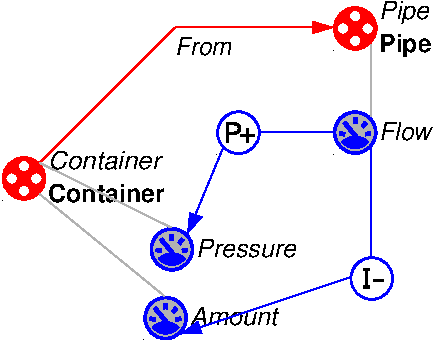
\includegraphics[scale=0.5]{cv_fromcontpipe-crop.pdf}
}
\subfigure{
    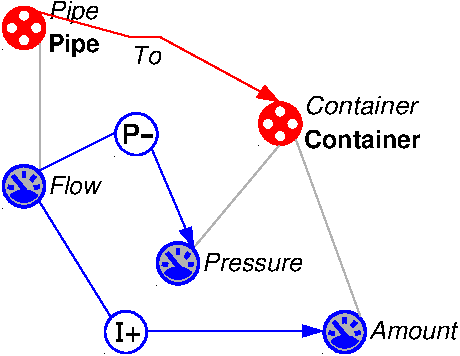
\includegraphics[scale=0.5]{cv_topipecont-crop.pdf}
}
\subfigure{
    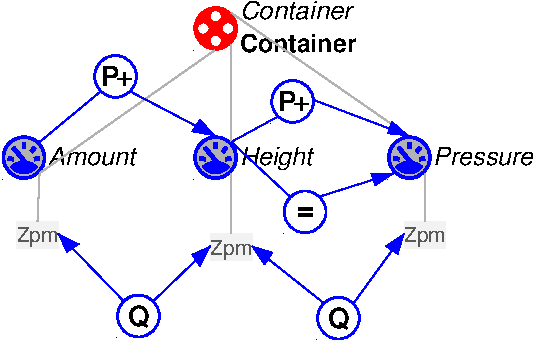
\includegraphics[scale=0.5]{cv_selfcontainer-crop.pdf}
}
\subfigure{
    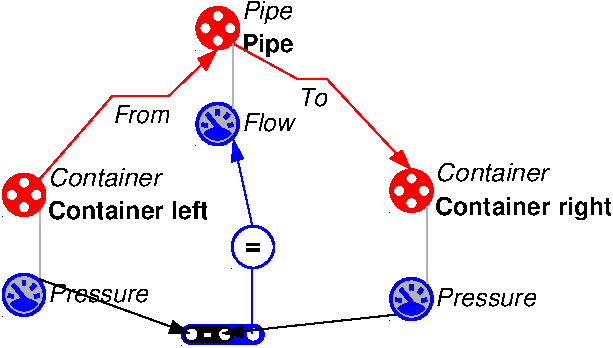
\includegraphics[scale=0.5]{cv_unfragment-crop.pdf}
}

\caption{After minimization on entities: four model compositional fragments for communicating vessels.}
\label{cv_frags2}
\end{figure}

Three communicating vessels.
%more text

\begin{comment}
\begin{verbatim}
Input:
[dependency(inf_pos, flow3, amount5), 
dependency(inf_neg, flow3, amount4), 
dependency(prop_neg, flow3, pressure5), 
dependency(prop_pos, flow3, pressure4), 
dependency(prop_pos, height4, amount4), 
dependency(prop_pos, height5, amount5), 
dependency(prop_pos, pressure5, height5), 
dependency(prop_pos, pressure4, height4), 
dependency(q_correspondence, height5, amount5), 
dependency(q_correspondence, pressure4, height4), 
dependency(q_correspondence, pressure5, height5), 
dependency(q_correspondence, height4, amount4), 
dependency(equals, flow3, min(pressure4, pressure5)), 
dependency(equals, height4, pressure4), 
dependency(equals, height5, pressure5), 
dependency(inf_pos, flow4, amount6), 
dependency(inf_neg, flow4, amount5), 
dependency(prop_neg, flow4, pressure6), 
dependency(prop_pos, flow4, pressure5), 
dependency(prop_pos, height6, amount6), 
dependency(prop_pos, pressure6, height6), 
dependency(q_correspondence, height6, amount6), 
dependency(q_correspondence, pressure6, height6), 
dependency(equals, flow4, min(pressure5, pressure6)), 
dependency(equals, height6, pressure6)]

Set of struct rels: 
[ (self, flow, flow), (self, amount, amount), (self, amount, height), 
(self, amount, pressure), (self, height, height), (self, height, pressure),
(self, pressure, pressure), (from, amount, flow), (from, height, flow), 
(from, pressure, flow), (to, flow, amount), (to, flow, height), 
(to, flow, pressure)]

Fragments (6):
[ (self, amount, height), 
	dependency(prop_pos, height, amount), 
	dependency(q_correspondence, height, amount)]
[ (self, height, pressure), 
	dependency(prop_pos, pressure, height), 
	dependency(q_correspondence, pressure, height), 
	dependency(equals, height, pressure)]
[ (from, amount, flow), dependency(inf_neg, flow, amount)]
[ (from, pressure, flow), dependency(prop_pos, flow, pressure)]
[ (to, flow, amount), dependency(inf_pos, flow, amount)]
[ (to, flow, pressure), dependency(prop_neg, flow, pressure)]

Unfragment:
[dependency(equals, flow3, min(pressure4, pressure5)), 
dependency(equals, flow4, min(pressure5, pressure6))]
\end{verbatim}
\end{comment}


%\subsection{Population dynamics}
%single population? split into birth, migration etc.
%interacting populations? but ants garden is too much

%more text
%TBD.

\section{Discussion}
We will now discuss several possible extensions both to model induction in
general and to model minimization in particular.
%more text

\subsection{Model minimization}

%more text

\subsubsection{Modular fragments as input}

Currently the implementation expects a single monolithic model as input, since
that is the output as given by the automated modeling algorithm. However, this
requirement could be lifted to allow partially modular fragments as input,
which is especially useful when the minimization algorithm is applied as part
of an interactive modeling assistant.

This could be implemented by finding a way to merge these fragments into a
monolithic fragment, while avoiding undergeneration by exploding all
dependencies to specific dependencies between instances. Such an extension is
fairly trivial but has not been implemented yet.

\subsubsection{Inheritance: hierarchy of fragments in output}

The output of our algorithm consists of a flat list of model fragments, but a
more advanced method would turn this into an inheritance hierarchy, to avoid
duplication and to increase re-use and clarity.

\subsection{Model induction}

\subsubsection{Conditions}

The induction algorithm has no support for conditions, except for
copying structural relations between entities as found in the scenario. This
severly limits the scope of models that can be induced. However, adding the
induction of conditions increases the complexity greatly. This is demonstrated
by an analogy to the Chomsky Hierarchy: with every addition of
context-sensitivity, the complexity increases, until it reaches Turing
equivalence in the unrestricted case. The Garp models that can currently be
induced are the subset of possible models such that only structural relations
can serve as conditions. 

On top of that, it only makes sense to add conditions to fragments, which
implies that splitting into fragments (but not minimizing) would need to be
integrated into the model induction algorithm itself instead of as a
transformation as has been presented in the current project.

\subsubsection{Interactivity}

The current requirement for the induction to have access to a perfect behavior
graph makes the algorithm virtually useless for practical purposes, because
such a behavior graph is very difficult to specify without already having a
qualitative model, which makes for a vicious circle. An alternative would be
to make the induction interactive. The algorithm would formulate a series of
maximally informative questions (comparable to automatic diagnosis
\cite{dekleerdiag}), employing the user as an informant. A series of
iterations can be performed, presenting the resulting behavior graph to the
user who can then highlight errors.

\subsubsection{Negative exemplars}

This brings us to the related problem of negative exemplars. Humans probably
have an idea not only of what a system does, but also what it does not do
(constraints). Negative exemplars are of course the very reason for the
problem of induction in philosophy \cite{hume, popper}.
However, since qualitative models are a formalization of human knowledge, not
induced from naturalistic data, negative exemplars are a resource that should
be exploited. Negative exemplars could be presented by the user in the form of
(in)equalities and as a list of impossible combinations of values.

\subsubsection{Inductive Logic Programming}

An alternative approach to model induction would be to use the general
framework of Inductive Logic Programming (ILP) \cite{mitchell}. This framework
provides a way to learn arbitrary Prolog programs based on background knowledge
and exemplars of predicates. In the case of inducing a Garp model this would
mean having the Garp engine as background, the behavior graph as the set of
exemplars, and model fragments represented as Prolog predicates (an encoding
would need to be defined) as output. In \cite{kuipers} (pp. 356 and on) a
method of axiomatizing qualitative models is discussed, in which state
transitions are first-order derivable theorems; this work could provide a good
starting point for an exploration of applying ILP to automated modeling.


% World domination etc.

\section{Conclusion}

Model minimization has been fruitfully applied to qualitative models. Our
approach is general enough that it applies both to Automatic Modeling and to
models made by beginners. From now on, minimizing qualitative models in Garp
can be done automatically, at least for the subset of models supported by the
proof of concept implementation. Further work on inducing models lies ahead
and given the results on inducing constraint models this work would seem to
have ample room for success.
%more text

\begin{thebibliography}{99}

% 1,5 - 2 pp. per artikel
\bibitem{newell} Allen Newell and Herbert A. Simon, ``Computer Science as
Empirical Inquiry: Symbols and Search,'' Communications of the ACM. vol. 19,
No. 3, pp. 113-126, March, 1976. \url{http://www.rci.rutgers.edu/~cfs/472
html/AI SEARCH/PSS/PSSH1.html}

%allebei
\bibitem{bredeweg-eco} Bredeweg, B. and Salles, P. (2009), Handbook of
Ecological Modelling, Chapter 19 - Mediating conceptual knowledge using
qualitative reasoning. In: J\/orgen, S.V., Chon, T-S., Recknagel, F.A. (Eds.),
Handbook of Ecological Modelling and Informatics. Wit Press, Southampton, UK,
pp. 351.398.

%allebei
\bibitem{bredeweg-garp} Bredeweg, B., Linnebank, F., Bouwer, A. and Liem, J.
(2009) 02 Bredeweg EtAl ECOINF 2009.pdf (598.325 Kb) Garp3 - Workbench for
Qualitative Modelling and Simulation. Ecological Informatics 4(5-6), 263-281.

%hanne
\bibitem{forbus} Forbus, K.D. (1984) Qualitative process theory. Artificial 
Intelligence, 24:85-168. 

\bibitem{forbus12} Forbus, K.D. (1993) Qualitative process theory: twelve years
after. Artificial Intelligence, 59:115-123. 

%andreas
\bibitem{kleer} Kleer, J. de and Brown J.S. (1984) deKleerBrown1984.pdf (4.005
Mb) A qualitative Physics based on confluences, Artificial Intelligence,
24:7-83 %(for the course you may ignore section 6)

%andreas
\bibitem{cioaca} Cioaca, Linnebank, Bredeweg, Salles 2009 Cioaca EtAlECOINF
2009.pdf (1,001.442 Kb) A qualitative reasoning model of algal bloom in the
Danube Delta Biosphere Resere (DDBR) in: \emph{ecological informatics 4} (2009)
p282-298

%hanne
\bibitem{buisman} Buisman, H., ``Automated modeling in process-based
qualitative reasoning''
\url{http://staff.science.uva.nl/~bredeweg/pdf/BSc/20062007/Buisman.pdf}

% (samenvatting van Buisman plus verbeteringen)
%hanne 
\bibitem{liem} Liem, J., Buisman, H. and Bredeweg, B., ``Supporting
Conceptual Knowledge Capture Through Automatic Modelling''

%hanne
\bibitem{vanweelden} van Weelden, C., ``Automated modeling of conceptual
knowledge'' \url{http://staff.science.uva.nl/~bredeweg/pdf/BSc/20082009/vanWeelden.pdf}

\bibitem{mitchell}
	Mitchell, Tom (1997), ``Machine Learning,'' McGraw Hill.

\bibitem{hopcroft}
	John Hopcroft and Jeffrey Ullman (1979). 
	``Introduction to Automata Theory, Languages, and Computation.'' Addison Wesley.

\bibitem{russellnorvig}
	Russell S, Norvig P (1995). 
	``Artificial Intelligence: A Modern Approach,'' 
	Prentice Hall Series in Artificial Intelligence. Englewood Cliffs, New Jersey

\bibitem[princesmolensky]
	Prince, Alan and Paul Smolensky (1993/2004): 
	``Optimality Theory: Constraint Interaction in Generative Grammar.''
	Blackwell Publishers (2004). Technical Report, Rutgers
	University Center for Cognitive Science and Computer Science
	Department, University of Colorado at Boulder (1993).

\bibitem{haugeland}
	Haugeland, John (1985), 
	``Artificial Intelligence: The Very Idea,''
	Cambridge, Mass.: MIT Press, ISBN 0-262-08153-9 .

\bibitem{smith}
	Barry Smith and Roberto Casati (1994)
	``Naive Physics: An Essay in Ontology.''
	{\em Philosophical Psychology}, 7/2, pp.\ 225-244.

\bibitem{dekleerdiag}
	De Kleer, J. and Williams, B. C. 1989. Diagnosis with behavioral modes.
	In \emph{Proceedings of the 11th international Joint Conference on Artificial
	intelligence - Volume 2} (Detroit, Michigan, August 20 - 25, 1989).
	International Joint Conference On Artificial Intelligence. Morgan
	Kaufmann Publishers, San Francisco, CA, 1324-1330. 

\bibitem{hume} 
	Hume, David (1910) [1748]. 
	``An Enquiry concerning Human Understanding.''
	P.F. Collier \& Son. 
	\url{http://18th.eserver.org/hume-enquiry.html#4}. 
	Retrieved 27 December 2007.

\bibitem{popper}
	Popper, Karl (1959). 
	``The Logic of Scientific Discovery.'' pp. Ch. 1. 
%	"...the theory to be developed in the following pages stands directly
%	opposed to all attempts to operate with the ideas of inductive logic."

\bibitem{kuipers}
	Kuipers, Benjamin (1994). ``Qualitative reasoning: modeling and simulation with incomplete knowledge,''
	MIT Press, ISBN	026211190X, 9780262111904

\end{thebibliography}

\end{document}

----------------------------------------------

Ideas

    * done: split code for model output into generation & garp adding
    * done: compositional model fragments 
    * deferred: (also: accept existing model fragments as input)
    * deferred: lift full envisionment requirement, accept negative input (eg. list of impossible value combinations).
    * deferred: user interaction: graphical dialog to choose best model in case of ambiguity

----------------------------------------------
Todos

    * done: fix influences
    * done: fix output of models to garp. deferred: each possible model should become a model fragment (too much ambiguity)
    * done: split into multiple model fragments: working code: qrsplit
    * done: collapse similar model fragments into generic model fragments (eg. Faucet1 =>I+ Bath1 and Faucet2 => I+ Bath2 becomes Faucet =>I+ Bath)
    * done: detect necessary structural relations / other conditions required to make a model fragment generic.
    * done: try other models listed in van Weelden & Buisman. notably, communicating vessels
    * distinguish between static (no influences) & process; filter current list of fragments and split them in a static and a process list.
    * integrate code with model induction (input) & garp (output)
	* input directly from AM database instead of coded by hand: hgp file is an XPCE object, look in /tmp (.pl source) 
	* output of minimized (split) models to garp.

    * report: 
	- Intro 
	- Summary per paper (literature review) 
	- Discussion 
	- Conclusion 
	- Project 
	- Theoretical / Practical / Technical Perspectives 
	* further details: blackboard

----------------------------------------------

Minutes
April 13th 2010

New plan:

    * Some sort of standard for what a well-formed fragment should be
    * -- Static vs process fragments?
    * -- Everything per entity 1 fragment?
    * -- Things like 'birth', 'death', 'emigration' and 'immigration'?
    * -- Influences?

    * We need some sort of evaluation to check our models against.

    * First run a the models we want to use and analyze their current output, compare them to our 'ideal' output.
    * We should not worry about intergration with the current Automatic Modeling code for now. First focus on hand-corrected input.
    * Recognizing duplicate (super)cluster could be a nice step to start with.. to get working on the code.

Notes:

    * Influences: now written to screen --> should be asserted
    * I's wrong direction? (inf-pos-a-b = b --> a)
    * naive dependencies: exponential
    * Communicating vessels: hack in causal groups: same entities (same_object_group/2)
    * Choose hacks for conceptually best model

    * Discussed with Floris that finding correspondences could be done faster by first looking for them without considering naive_dependencies yet.


----------------------------------------------

Requirements for the thesis:

 

1) The thesis consists of two parts, a literature review and a project report.

Both parts can be done in pairs or individually if this is preferred. In the
end each student should submit one integrated document. (Note that this makes
life easier: in your report you will be able to refer to concepts discussed in
the review.)

The total amount of pages should be around 30, figures included, with each part
taking about half. (Note that in general less pages may be better if all
arguments are still explicit and clear, but this is also harder in practice.
So, aim for making your points clearly and logically without unnecessary
words.)

2) The literature overview of the papers (or sections of papers) we've
discussed in class should be a scientific review, and it should show that
you've read and understood them.

A possible approach is to start with a general introduction, then summarize and
discuss each paper, and then end with a short conclusion of the papers.

The level of detail should be in between the paper itself and an abstract.
Saying state graphs are generated by a procedure is too general, listing the
steps in the procedure is too detailed. Instead give the general idea of the
procedure and discuss its properties, pros and cons.

(Hints, but not requirements: a) It is nice if you can link the papers together
in your discussion. b) It is also nice if you can use the review to introduce
the problem area of your project research. c) Note that the papers we've
discussed each have different perspectives: theoretical, technical,
application/modeling)

3) The report on your project should be like a scientific research paper and it
should be provide sufficient detail such that someone else could replicate your
work. Be sure to make all your assumptions, choices and reasoning steps
explicit.

4) If you want feedback you can submit initial versions of papers for feedback.
Allow for a couple of days for reading of course, and I will provide mainly
overall feedback on whether you're moving in the right direction or which other
approach you could take. Still this should save you time and effort, so take
the opportunity!

5) The final deadline for the thesis is Friday the 28th of May, 18:00 hours.

NB This deadline is solid as a rock, no exceptions, so evade Murphy's law and
plan in some reserve time.

Last but not least: Good Luck, Start in Time, & Have Fun!


